\documentclass{article}

\usepackage[spanish]{babel}
\usepackage{lipsum}
\usepackage{graphicx}
\usepackage{mathtools}
\usepackage[style=apa]{biblatex}
\addbibresource{referencias.bib}

\title{Mi primer articulo}
\author{Gerardo Becerra}
\date{\today}

\begin{document}
  \maketitle

  \begin{abstract}
    \lipsum[1]
  \end{abstract}

  \section{Introducción}
  \lipsum[1-2] \cite{goodfellow2016deep}

  \begin{itemize}
    \item Primer elemento de la lista
    \item Segundo elemento de la lista
    \item Tercer elemento de la lista
    \begin{enumerate}
      \item Elemento 1
      \item Elemento 2
      \item Elemento 3
    \end{enumerate}
    \item Cuarto elemento de la lista
  \end{itemize}

  \lipsum[3-4]

  \section{Metodología}
  \lipsum[1] \cite{PIGA2021415}
  \begin{figure}
    \centering
    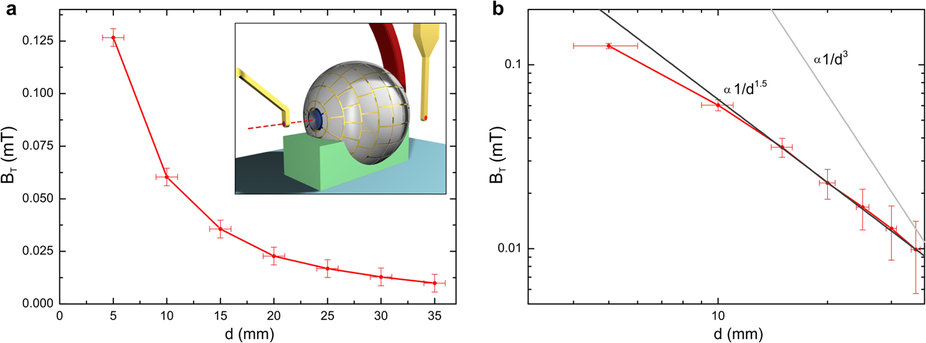
\includegraphics[width=\textwidth]{image.jpg}
    \caption{A Magnetic Wormhole.}
  \end{figure} 
  \lipsum[2]\footnote{Este es un pie de página.}
  Los datos de los estudiantes se encuentran disponbibles en la tabla \ref{tab:estudiantes}.

  \begin{table}[h]
    \centering
    \begin{tabular}{|l||cr|}
      \hline
      Nombre & Edad & Ciudad\\
      \hline
      Juan & 25 & Cali\\
      Ana & 32 & Pasto\\
      \hline
    \end{tabular}
    \caption{Datos de los estudiantes.}
    \label{tab:estudiantes}
  \end{table}
  \lipsum[3]


  \section{Resultados}
  \lipsum[1] \cite{9372789}

  \begin{equation*}
    A_{m,n} = 
    \begin{pmatrix}
      a_{1,1} & a_{1,2} & \cdots & a_{1,n} \\
      a_{2,1} & a_{2,2} & \cdots & a_{2,n} \\
      \vdots  & \vdots  & \ddots & \vdots  \\
      a_{m,1} & a_{m,2} & \cdots & a_{m,n} 
    \end{pmatrix}
  \end{equation*}

  \lipsum[3-4] \cite{9372789}
  
  \section{Conclusiones}
  \lipsum[1-4]
 
  \printbibliography
\end{document}